\documentclass[14pt]{extreport}
\usepackage{authblk}
\usepackage[utf8]{vietnam}
\usepackage{amsmath}
\usepackage{amsfonts}
\usepackage{amssymb}
\usepackage{graphicx}
\usepackage{longtable}
\usepackage{multirow}
\usepackage[english]{babel}
\usepackage[utf8]{inputenc}
\usepackage{fancyhdr}
\usepackage{float}
\usepackage[table,xcdraw]{xcolor}

%---------------------------------------------------------
\pagestyle{fancy}
\fancyhf{}
\rhead{\rightmark}
\rfoot{Page \thepage}
\title{Đồ án về giải thuật nén Huffman}
\author{Vu Cong Duy - 19120212

Nguyen Hoang Anh Kiet - 19120266

To Gia Thuan - 19120389
}
\date{January 2021}


\begin{document}
\maketitle

\chapter{Giới thiệu}
\section{Vấn đề về việc nén dữ liệu}

Từ những ngày đầu của kỷ nguyên công nghệ thông tin, việc nén thông tin để tiết kiệm dung lượng lưu trữ đã là một đề tài được đem ra thảo luận rất sôi nổi.

Trong đó, David A. Huffman đã cho ra đời một thuật toán đơn giản, dễ cài đặt và tính hiệu quả cao được đặt tên theo chính ông - thuật toán Huffman.

Thuật toán được đề xuất khi ông còn là sinh viên Ph.D. tại MIT, và công bố năm 1952 trong bài báo "A Method for the Construction of Minimum-Redundancy Codes". Sau này Huffman đã trở thành một giảng viên ở MIT và sau đó ở khoa Khoa học máy tính của Đại học California, Santa Cruz, Trường Kỹ nghệ Baskin (Baskin School of Engineering). 

Thuật toán nén Huffman là 1 thuật toán mã hoá thông tin dùng để nén dữ liệu dựa trên việc tối ưu hoá việc mã hoá các kí tự trong chuỗi ban đầu bằng việc xây dựng bộ mã nhị phân đại diện cho từng kí tự trong đó. Thuật toán có mục tiêu sẽ xây dựng được bảng mã nhị phân đại diện cho từng kí tự sao cho những kí tự có tần suất xuất hiện nhiều sẽ có mã nhị phân đại diện cho nó ngắn và ngược lại.
\section{Tại sao ta có thể nén được dữ liệu?}
Các con chữ (kí tự) chúng ta thường hay sử dụng trong văn bản trên máy tính được hiển thị dựa trên bộ mã kí tự ASCII (gồm 256 kí tự). Vì thế, mỗi kí tự được biểu diễn bởi 8 bit ( $2^8 =256$)

Sở dĩ mỗi kí tự phải đủ 8 bit là để chúng có thể được phân biệt vời 255 kí tự còn lại. Tuy nhiên, trong một văn bản thông tin, hiếm khi nào ta sử dụng hết 256 kí tự. Vì thế, một câu hỏi được đặt ra là : liệu có cần dùng tới 8 bit để có thể phân biệt các kí tự với nhau không khi mà số kí tự thực tế sử dụng là rất ít.

Hầu hết mọi hệ điều hành đọc các ký tự vẫn yêu cầu phải biểu diễn dưới dạng 8 bit. Nhưng nếu xét trên phương diện lưu trữ, việc dùng số bit ít hơn 8 để biểu diễn ký tự vẫn đảm bảo được tính toàn vẹn của dữ liệu (và tất nhiên là tiết kiệm bộ nhớ hơn). Đây cũng chính là cơ sở của thuật toán Huffman
\chapter{Cách thực hoạt động}
\section{Ý tưởng chính}

\subsection{Làm rõ việc thay thế bảng mã ASCII để biểu diễn}
Để mã hóa các kí hiệu (kí tự, chữ số, ...) ta thay chúng bằng các xâu nhị phân, được gọi là từ mã của kí hiệu đó. Chẳng hạn bộ mã ASCII, mã hóa cho 256 kí hiệu là biểu diễn nhị phân của các số từ 0 đến 255, mỗi từ mã gồm 8 bít. Trong ASCII từ mã của kí tự "a" là 1100001, của kí tự "A" là 1000001. Trong cách mã hóa này các từ mã của tất cả 256 kí hiệu có độ dài bằng nhau (mỗi từ mã 8 bít). Nó được gọi là mã hóa với độ dài không đổi. 

 Khi mã hóa một tài liệu có thể không sử dụng đến tất cả 256 kí hiệu. Hơn nữa trong tài liệu chữ cái "a" chỉ có thể xuất hiện 1000000 lần còn chữ cái "A" có thể chỉ xuất hiện 2, 3 lần. Như vậy ta có thể không cần dùng đủ 8 bít để mã hóa cho một ký hiệu, hơn nữa độ dài (số bít) dành cho mỗi kí hiệu có thể khác nhau, kí hiệu nào xuất hiện nhiều lần thì nên dùng số bít ít, ký hiệu nào xuất hiện ít thì có thể mã hóa bằng từ mã dài hơn. Như vậy ta có việc mã hóa với độ dài thay đổi.
 
 \subsection{Ví dụ}
\cite{1}Để làm rõ, ta đi đến ví dụ sau : 

Cho một đoạn tập tin có dữ liệu là : ABCDBADA

Ta tạo các dãy bit mới để biểu diễn các ký tự thay cho bảng ASCII. (Cách tạo sẽ được làm rõ ở phần sau)

\begin{center}
    \begin{figure}[H]
    \begin{center}
     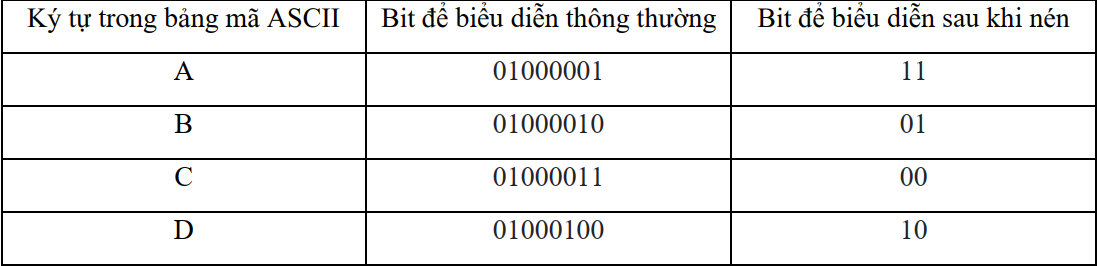
\includegraphics[scale=.65]{zip_table.PNG}
    \end{center}
    \caption{Dãy bit biểu diễn ký tự}
    \label{refhinh1}
    \end{figure}
\end{center}


Với cách lưu trữ thông thường thì cần: 8 (ký tự) * 8 bit = 64 bit = 8 byte để lưu trữ.

\textbf{ABCDBADA\\
01000001 01000010 01000011 01000100 01000010 01000001 01000100 01000001
}


Thực tế văn bản chỉ có 4 chữ cái A,B,C,D nên chỉ cần 2 bit cho mỗi kí tự, cần: 8 (ký tự) * 2 bit = 16 bit = 2 byte để lưu trữ.

\textbf{ABCDBADA\\
11 01 00 10 01 11 10 11\\
Ò
}

Trong máy tính chỉ lưu theo byte, tức là những số bit lẻ cần phải được thêm vào để cho đủ 1 byte (8 bit). Ví dụ trên giả định rằng thông tin cần thiết cho việc giải nén được lưu trữ và xử lý riêng, nên phương pháp nén Huffman giúp giảm đi 75\% (2 byte so với 8 byte) dung lượng lưu trữ đối vói đoạn văn bản trong ví dụ. Những đoạn mã thu gọn sau khi nén được gọi là mã Huffman.
Để tạo ra mã Huffman, cấu trúc dữ liệu cây nhị phân tìm kiếm được áp dụng, được gọi là cây Huffman.
\section{Chi tiết cách nén}
Ở phần này, từng bước sẽ được minh họa dựa vào ví dụ ở phần trước : Nén dãy ký tự \textbf{ABCDBADA}
\subsection{Bước 1: Lập bảng tần số}
Đếm số lượng xuất hiện của từng ký tự có trong văn bản, bao gồm cả các ký tự đặc biệt như ký tự xuống dòng (\textbackslash n), ký tự null (\textbackslash 0) hay ký tự khoảng cách.

\begin{center}
    \begin{figure}[H]
    \begin{center}
     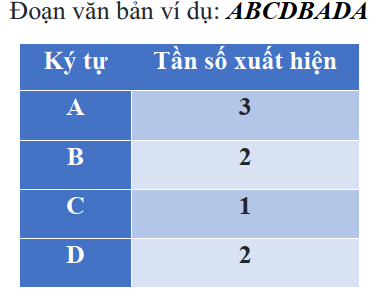
\includegraphics[scale=.65]{sequence_table.PNG}
    \end{center}
    \caption{Ví dụ bảng tần số}
    \label{refhinh1}
    \end{figure}
\end{center}

Cách cài đặt ở bước này tương đối đơn giản : ta tạo một mảng với các phần tử có cấu trúc gồm ký tự, tần số xuất hiện của ký tự đó và dãy bit để biểu diễn ký tự đó ( dữ liệu này sẽ được thiết lập vào các bước sau).
\begin{center}
    \begin{figure}[H]
    \begin{center}
     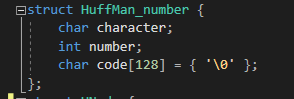
\includegraphics[scale=2.0]{Huffman_number.PNG}
    \end{center}
    \caption{Hàm lập bảng tần số}
    \label{refhinh1}
    \end{figure}
\end{center}

\begin{center}
    \begin{figure}[H]
    \begin{center}
     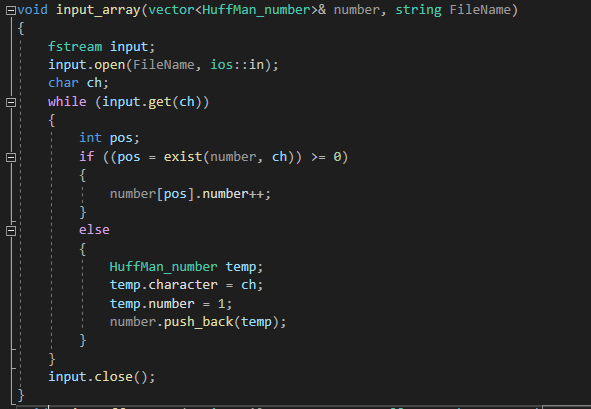
\includegraphics[scale=1.0]{input_array.PNG}
    \end{center}
    \caption{Hàm lập bảng tần số}
    \label{refhinh1}
    \end{figure}
\end{center}
\subsection{Bước 2: Xây dựng cây Huffman}
*Yêu cầu trước khi thực hiện : cài đặt các giải thuật cho hàng đợi ưu tiên của nút dựa với chỉ số sắp xếp là tần số xuất hiện.

\begin{center}
    \begin{figure}[H]
    \begin{center}
     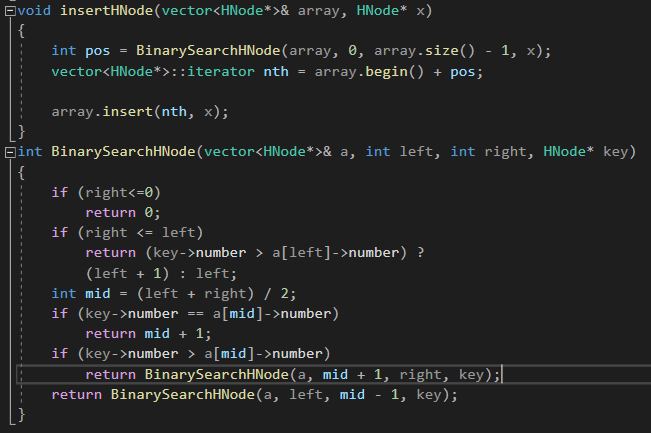
\includegraphics[scale=1.]{priority_queue.PNG}
    \end{center}
    \caption{Cài đặt hàng đợi ưu tiên}
    \label{refhinh1}
    \end{figure}
\end{center}

Bước đầu để có thể tạo dãy bit cho từng ký tự chính là xây dựng cây Huffman dựa vào tần số của từng ký tự. Cây Huffman là một cấu trúc heap với nút cha lớn hơn nút con. Các node bao gồm phần dữ liệu, tần số, nút con trái và nút con phải.

1. Ta tiến hành tạo các nút từ bảng tần số ở bước 1 đã lập. Sau đó đưa chúng vào hàng đợi ưu tiên (xếp từ bé đến lớn).

\begin{center}
    \begin{figure}[H]
    \begin{center}
     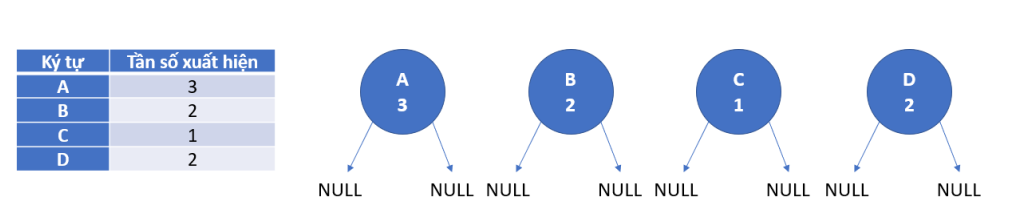
\includegraphics[scale=0.65]{createNode.PNG}
    \end{center}
    \caption{Tạo node từ bảng tần số}
    \label{refhinh1}
    \end{figure}
\end{center}

2. Dequeue 2 node từ hàng đợi ưu tiên ( cũng chính là 2 node có tần số bé nhất), tạo một nút cha có tần số là tổng tần số 2 nút con, dữ liệu của nút cha là chuỗi ghép từ chuỗi của 2 node con. Sau đó enqueue nút cha vào hàng đợi ưu tiên ( tức cho node cha vào vị trí sao cho hàng đợi gồm các node vẫn được sắp xếp từ bé đến lớn theo tần số)

\begin{center}
    \begin{figure}[H]
    \begin{center}
     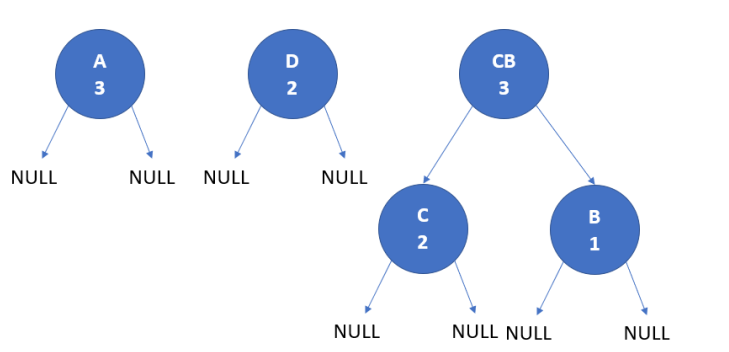
\includegraphics[scale=0.8]{createNode_1.PNG}
    \end{center}
    \caption{Tạo node cha và enqueue vào priority queue}
    \label{refhinh1}
    \end{figure}
\end{center}

3. Lặp lại bước đầu cho đến khi hàng đợi chỉ còn lại 1 phần tử, đó cũng chính là nút gốc của cây Huffman.

\begin{center}
    \begin{figure}[H]
    \begin{center}
     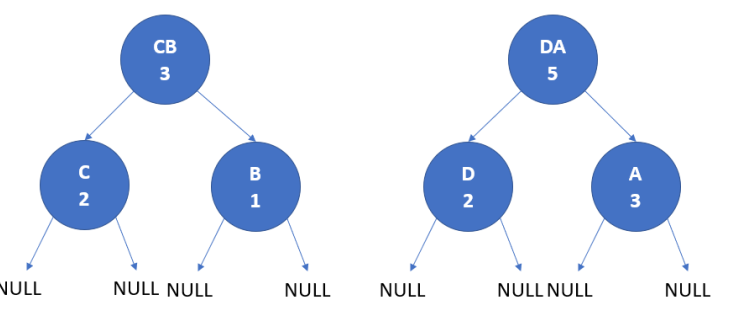
\includegraphics[scale=0.7]{createNode_2.PNG}
    \end{center}
    \caption{Tiếp tục vòng lặp}
    \label{refhinh1}
    \end{figure}
\end{center}

\begin{center}
    \begin{figure}[H]
    \begin{center}
     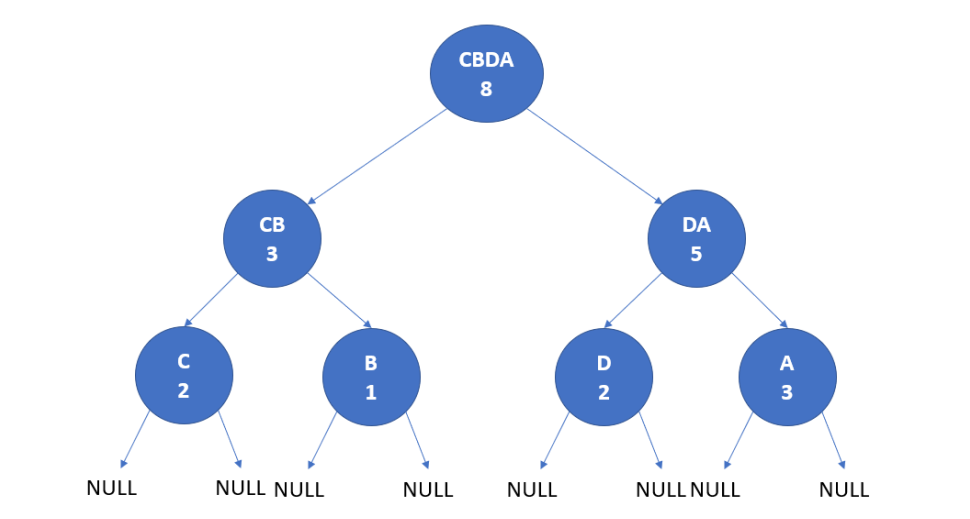
\includegraphics[scale=0.65]{createNode_3.PNG}
    \end{center}
    \caption{Phần tử còn lại duy nhất trong hàng đợi là nút gốc của cây nhị phân Huffman}
    \label{refhinh1}
    \end{figure}
\end{center}

\begin{center}
    \begin{figure}[H]
    \begin{center}
     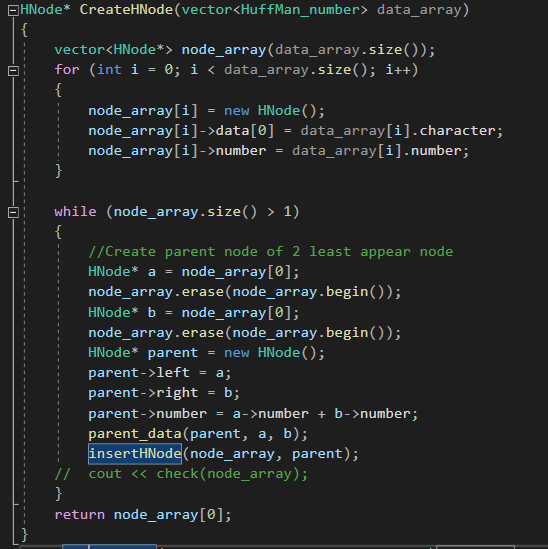
\includegraphics[scale=1.35]{createNode_source.PNG}
    \end{center}
    \caption{Mã nguồn tạo Hnode}
    \label{refhinh1}
    \end{figure}
\end{center}
\subsection{Bước 3: Điền dãy cho cho từng ký tự}
Dưa trên cây Huffman đã tạo ở bước 2, ta duyệt cây Huffman để tìm ra chuỗi bit của từng ký tự.

Chuỗi bit của ký tự dựa vào đường đi từ nút gốc đến nút lá chứa ký tự đó. Ta tìm kiếm nút lá chứa ký tự bằng cách dò tìm xem ký tự đó nằm trong chuỗi ký tự của nút con bên trái hay bên phải, nếu bên trái thì tiếp tục tiếp kiếm với nút gốc là nút bên trái, bên phải tương tự. Với mỗi lần đi sang trái, ta thêm số 0 vào sau chuỗi, và sang phải là số 1. Lặp lại đến khi nào nút lá có chuỗi chính là kí tự ta cần tìm. 

\begin{center}
    \begin{figure}[H]
    \begin{center}
     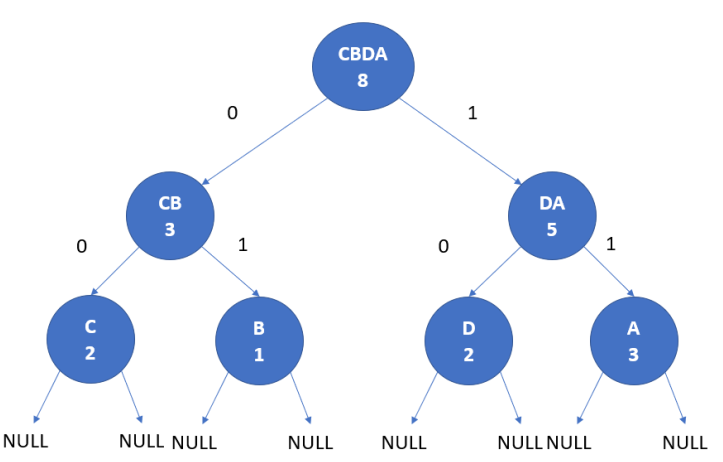
\includegraphics[scale=0.8]{get_code_1.PNG}
    \end{center}
    \caption{Minh hoa đường đi}
    \label{refhinh1}
    \end{figure}
\end{center}

\begin{center}
    \begin{figure}[H]
    \begin{center}
     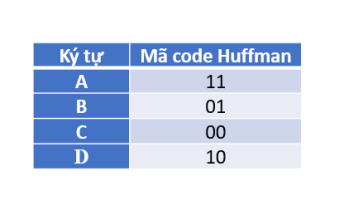
\includegraphics[scale=1.0]{get_code_2.PNG}
    \end{center}
    \caption{Chuỗi bit cho các kí tự sau khi thực hiện thuật toán}
    \label{refhinh1}
    \end{figure}
\end{center}

\begin{center}
    \begin{figure}[H]
    \begin{center}
     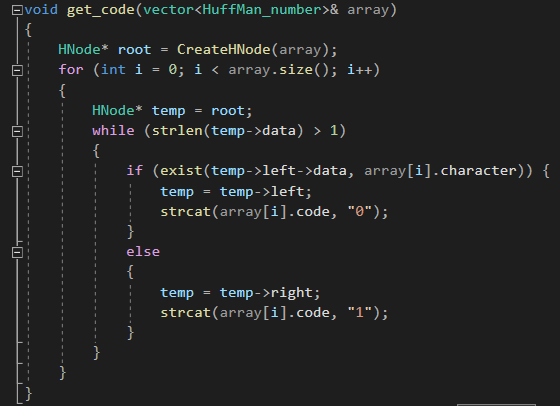
\includegraphics[scale=1.0]{get_code_source.PNG}
    \end{center}
    \caption{Mã nguồn lấy mã huffman cho tất cả các kí tự}
    \label{refhinh1}
    \end{figure}
\end{center}

\subsection{Bước 4: Tạo file nén}
File nén sẽ bao gồm 2 phần : bảng tần số và dữ liệu cần nén. Khi giải nén, bảng tần số sẽ được sử dụng để tạo dựng lại cây tìm kiếm Huffman.
Bảng tần số : có cấu trúc là <ký tự><ký tự ascii số 16><tần số>.\\Trong đó kí tự ascii số 16 dùng để nhận biết giữa <ký tự> và <tần số> trong trường hợp <ký tự> là một chữ số và do kí tự ascii số 16 không có trong nhập liệu.


Dữ liệu : duyệt từng ký tự trong tập tin, lưu mã bit tuần tự sao cho đủ 8 bit thì xuất ký tự đó ra tập tin nén. Do đó cần thực hiện các thao tác trên bit dữ liệu. Một số thao tác trên bit:
\begin{center}
    \begin{figure}[H]
    \begin{center}
     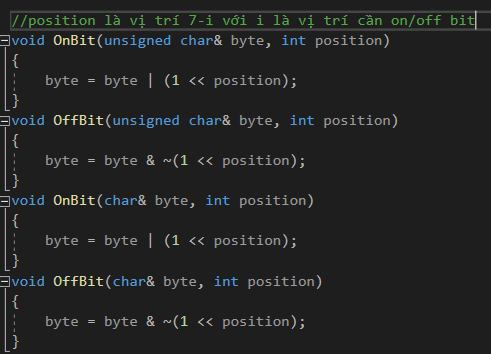
\includegraphics[scale=1.0]{bit on off.PNG}
    \end{center}
    \caption{Hàm thao tác bit}
    \label{refhinh1}
    \end{figure}
\end{center}

\begin{center}
    \begin{figure}[H]
    \begin{center}
     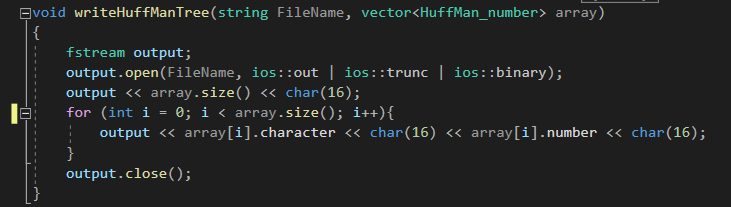
\includegraphics[scale=1.0]{write_huffman_tree.PNG}
    \end{center}
    \caption{Hàm ghi bảng tần số}
    \label{refhinh1}
    \end{figure}
\end{center}

\begin{center}
    \begin{figure}[H]
    \begin{center}
     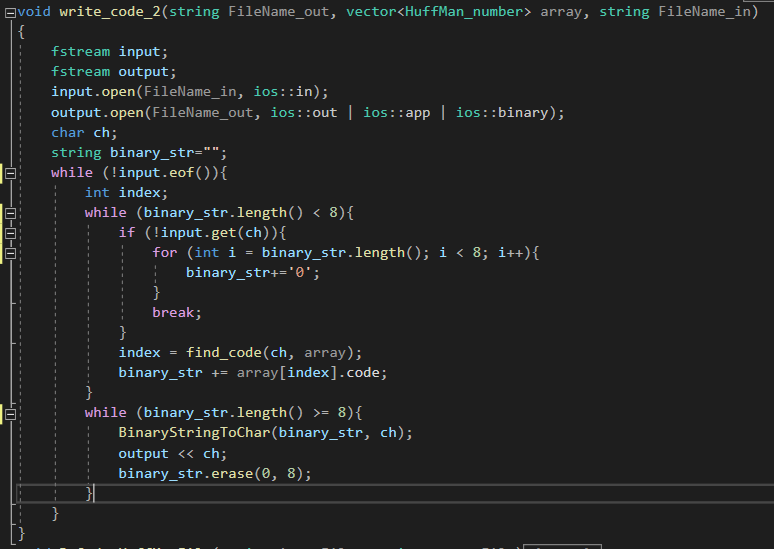
\includegraphics[scale=1.0]{write_code.PNG}
    \end{center}
    \caption{Hàm ghi dữ liệu}
    \label{refhinh1}
    \end{figure}
\end{center}
\section{Chi tiết cách giải nén}
Việc giải nén đơn giản hơn rất nhiều vì đã có sẵn các hàm từ việc nén và ta chỉ việc làm ngược lại khi nén.
1. Đọc bảng tần số
2. Xây dựng cây huffman từ bảng tần số (hàm có sẵn)
3. Phân mảnh kí tự trong phần dữ liệu ra thành các dãy bit, rồi dựa vào các dãy bit để dò tìm đến nốt lá chứa kí tự.

\begin{center}
    \begin{figure}[H]
    \begin{center}
     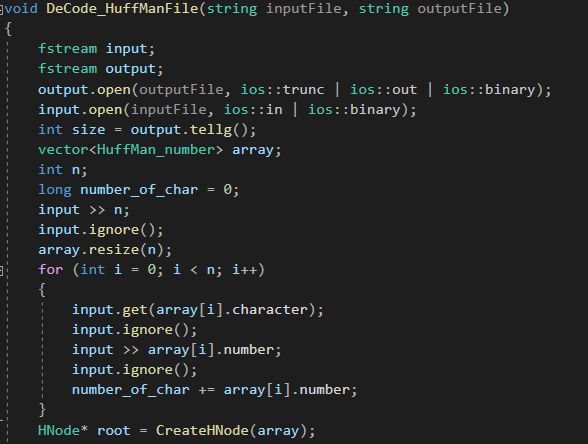
\includegraphics[scale=1.0]{decode_1.PNG}
    \end{center}
    \caption{Đọc bảng tần số}
    \label{refhinh1}
    \end{figure}
\end{center}

\begin{center}
    \begin{figure}[H]
    \begin{center}
     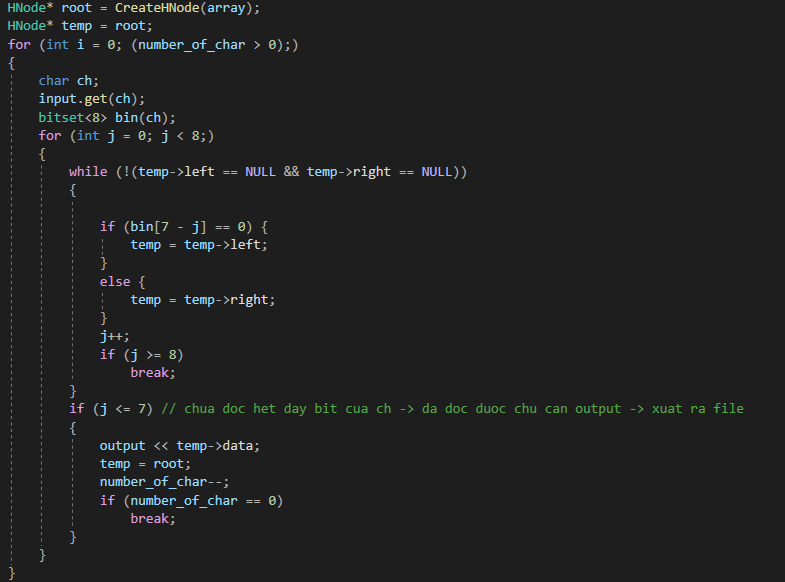
\includegraphics[scale=0.8]{decode_2.PNG}
    \end{center}
    \caption{Phân giải từ dữ liệu file nén}
    \label{refhinh1}
    \end{figure}
\end{center}
\section{Văn bản có kí tự ngoài bảng ASCII 8-bit}
Câu hỏi được đặt ra rằng liệu thuật toán Huffman có thể dùng cho các ngôn ngữ có những kí tự nằm bên ngoài bảng ASCII 8-bit như Tiếng Việt, Trung, Hàn,... không? Để giải đáp cho câu hỏi này, ta phải hiểu các bảng mã và quy tắc biểu diễn của các ngôn ngữ đó.

Đa số các ký tự đặc biệt hiện nay (và kể cả kí tự nằm trong bảng ASCII 8-bit) đều được biểu diễn bằng bảng mã UTF-8. Bảng mã UTF-8 biểu diễn các ký tự đặc biệt bằng dãy các byte (8-bit). Những byte này có thể biểu diễn các kí tự ở bảng mã ASCII.

\begin{center}
    \begin{figure}[H]
    \begin{center}
     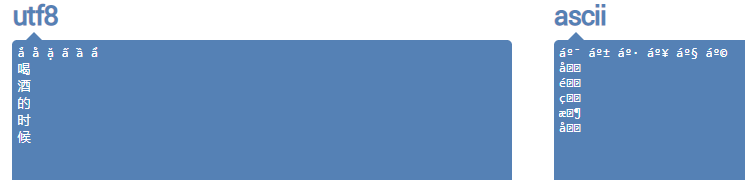
\includegraphics[scale=0.9]{utf8_ascii.PNG}
    \end{center}
    \caption{Các }
    \label{refhinh1}
    \end{figure}
\end{center}

Vì vậy, khi thực hiện thuật toán ta có thể xem các byte kí tự ấy là các byte kí tự riêng lẻ, mỗi byte kí tự riêng lẻ ấy đều được gán cho mã huffman khác nhau. Khi giải nén, các byte kí tự riêng lẻ ấy viết kề nhau thì chương trình sử dụng bảng mã UTF-8 sẽ tự nhận biết và biểu diễn kí tự đặc biệt ấy.
\chapter{Tổng kết}
\section{Độ phức tạp thuật toán}
Ta phân tích độ phực tạp dựa vào số kí tự cần nén. Gọi số kí tự cần nén là $n$. Số phép toàn cần thực hiện là $T(n)$
\subsection{Thuật toán nén}
Ở thuật toán nén, bước đầu tiên là phải duyệt file để xây dựng bảng tần số, ta cho mỗi lặp cần 1 phép toán để đọc vào bộ nhớ, số phép toán thực hiện : 

$$n$$

Các bước để xây dựng mã Huffman cho từng kí tự được cho là rất nhỏ bởi chỉ có thể có tối đa chưa đến 256 kí tự, vì vậy số phép toán là hữu hạn. Khi số kí tự cần nén $n$ lớn thì số phép toán hựu hạn ấy lại không đáng kể.

Tạo file nén cũng cần duyệt hết file để xây dựng file nén, số phép toán thực hiện : 

$$n$$

Vậy số phép toán của giải thuật Huffman là : 

$$T(n)\approx 2n = O(n)$$
\subsection{Thuật toán giải nén}
Gọi tỉ số nén là $\frac{1}{a}$ với $a \in N $. Ở lần duyệt file nén, ta có số lần lặp là : 

$$\frac{1}{a} . n$$

Các bước xây dựng mã Huffman như đã đề cập ở phần trên : không đáng kể.

Gọi kỳ vọng số lần đi sáng trái/phải trong cây nhị phân Huffman để tìm được kí tự cần ghi là $k$ với $k \in N $. Ở bước giải nén, số lần lặp là : 

$$k. n$$

Vậy số phép toán thực hiện ở bước giải nén là : 

$$T(n)\approx k.n + \frac{1}{a} . n = O(n)$$

\section{Độ hiệu quả thuật toán}
Để đánh giá độ hiệu quả thuật toán, ta dựa vào hệ số nén là thương của độ lớn file sau khi nén và trước khi nén.

Với văn bản của các ngôn ngữ mà các chữ các có trong bảng mã ASCII 8 bit như Tiếng Anh, Pháp, Đức, Ý, Tây Ban Nha,... thì tỉ số nén thấp, xấp xỉ 50\%

\begin{center}
    \begin{figure}[H]
    \begin{center}
     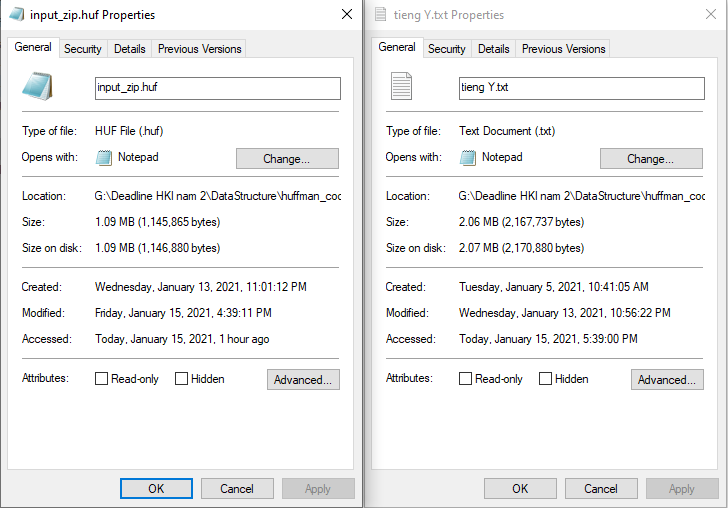
\includegraphics[scale=1]{tisonen_TiengY.PNG}
    \end{center}
    \caption{Tỉ số nén của văn bản Tiếng Ý : 52.9\%}
    \label{refhinh1}
    \end{figure}
\end{center}

Những văn bản mà các chứ không nằm trong bảng ASCII như Tiếng Việt, Trung, Hàn, Thái,... thì tỉ số nén cao, dao động trong khoảng 70\%
\begin{center}
    \begin{figure}[H]
    \begin{center}
     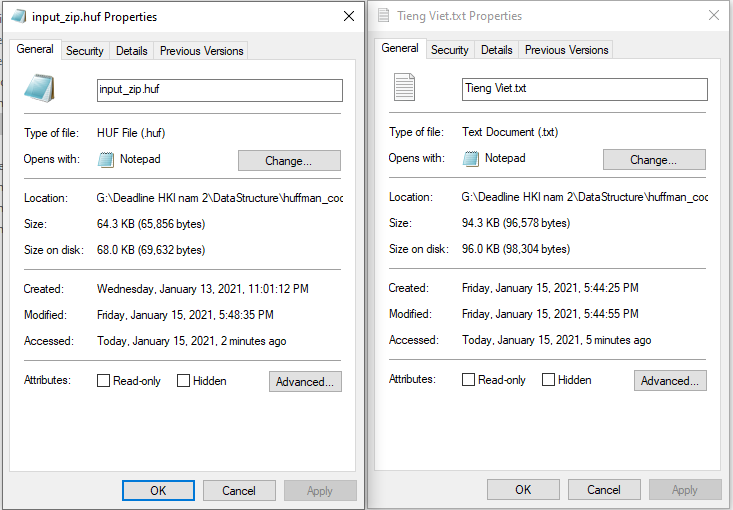
\includegraphics[scale=1]{tisonen_TiengViet.PNG}
    \end{center}
    \caption{Tỉ số nén của văn bản Tiếng Việt : 68.1\%}
    \label{refhinh1}
    \end{figure}
\end{center}

\begin{center}
    \begin{figure}[H]
    \begin{center}
     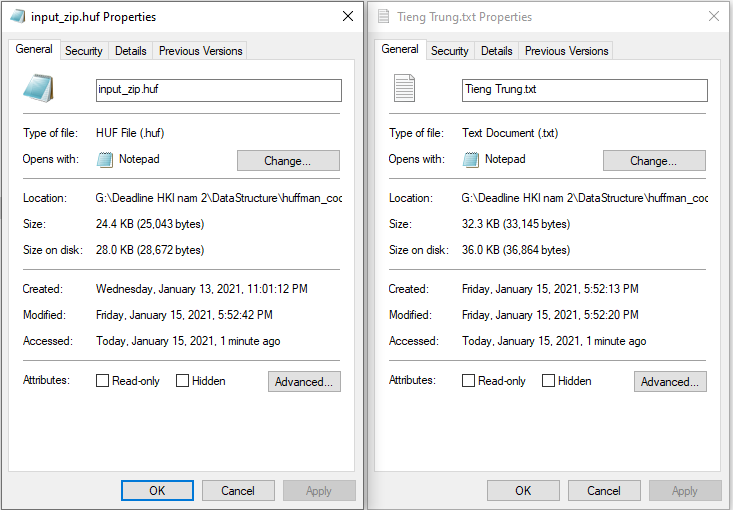
\includegraphics[scale=1]{tisonen_TiengTrung.PNG}
    \end{center}
    \caption{Tỉ số nén của văn bản Tiếng Trung : 75\%}
    \label{refhinh1}
    \end{figure}
\end{center}

\begin{thebibliography}{3}
\bibitem{1}Đại học Khoa học tự nhiên TPHCM . {\it Tài liệu hướng dẫn thực hành học phần CS104 – Cấu trúc dữ liệu - ITEC}. 2020.
\bibitem{2}Thomas H.Cormen  .{\it  Introduction to Algorithms}. 2009.
\bibitem{3}{https://vi.wikipedia.org/wiki/M\%C3\%A3\_h\%C3\%B3a\_Huffman}.

\end{thebibliography}
\end{document}
